At first, the results of the methods on single robots must be investigated
in order to evaluate the performance of the final localization algorithm.
Depending on the accuracy of the individual direction results, the quality
of the team decision is limited.

Primary, whistle sounds were recorded in the laboratory of the HULKs.
If not emphasized particularly, the height of the sound source is 1.5\si{m}.
% signal start detection evaluation
First, the result of the direction detection on one robot
is examined profoundly with one measurement as an example.
There, we focus on the correctness and precision of the different methods.
To investigate the final localization of the team, measurements were
done with five robots on a field.
At the end, all measurements are used to assess the methods in a general matter.

\subsection{\ac{TDOA} Methods}

For comparability of the results, the same measurements are taken into
account to analyse the \ac{TDOA} methods.
Part of the channel inputs of the whistle signal used in this section is plotted
in \ref{fig:04_tdoaSignal}.
Here, the sound source is placed -33.7\si{\degree} on the right front
of the robot with 4.5\si{m} distance.
% -------------------------------------------------------------
\begin{figure}[ht]
	\centering
		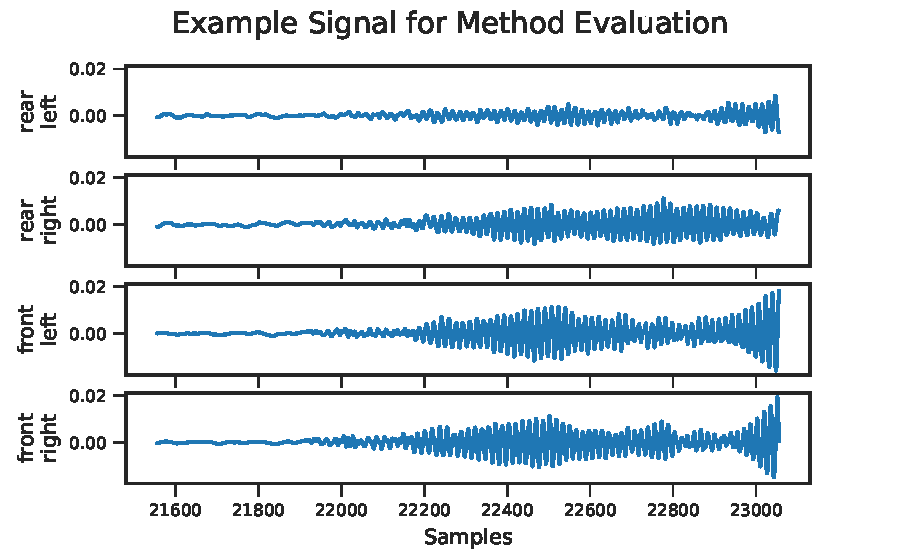
\includegraphics[]{figures/evaluation/cc_frontRight_1_signal}
	\caption{Signal start section of a whistle sound recorded from front right.}
	\label{fig:04_tdoaSignal}
\end{figure}
% -------------------------------------------------------------

The frames used for the \ac{CC} and \ac{GCC} methods are chosen in the same way
and are therefore equal.

\subsubsection{Cross Correlation}
% -------------------------------------------------------------
\begin{figure}[ht]
	\centering
		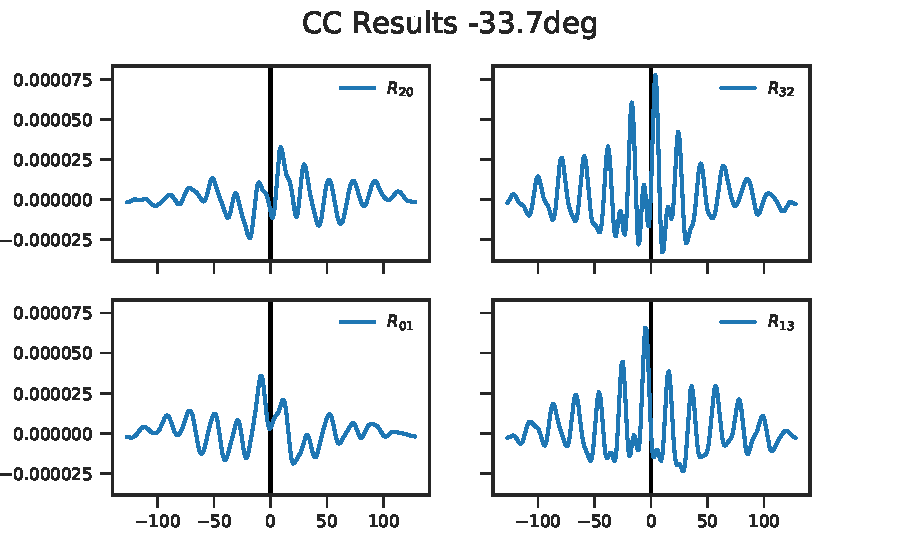
\includegraphics[]{figures/evaluation/cc_frontRight_1}
	\caption{Signal start section of a whistle sound recorded from front right.}
	\label{fig:04_tdoaSignal}
\end{figure}
% -------------------------------------------------------------

\subsubsection{Generalized Cross Correlation}
% -------------------------------------------------------------
\begin{figure}[ht]
	\centering
		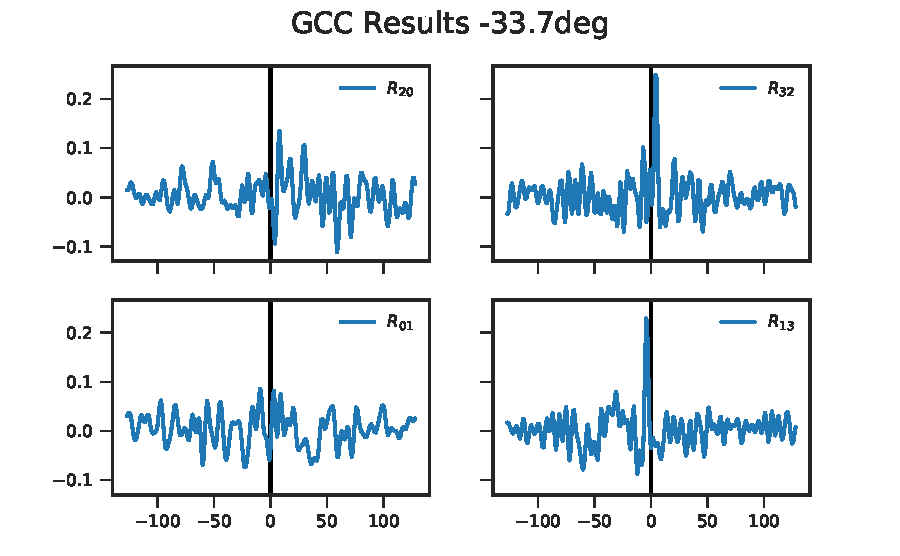
\includegraphics[]{figures/evaluation/gcc_frontRight_1}
	\caption{Signal start section of a whistle sound recorded from front right.}
	\label{fig:04_tdoaSignal}
\end{figure}
% -------------------------------------------------------------

\subsection{Team Decision Filter}

The size of the field used in this work is smaller than the regular \ac{SPL}
field. It's length is 7.5\si{m} and it's width is 5\si{m}.
It is looked at the result of one exemplary measurement where the behavior
of the team filter is of prime importance.
